\documentclass{article}
\usepackage{amsmath}
\usepackage{MnSymbol}
\usepackage{wasysym}
\usepackage{graphicx}
\usepackage{float}
\usepackage[export]{adjustbox}
\begin{document}
\begin{center}
\LARGE \bfseries{Answers to Problem Set 3}\\
 Group name: Ferienspass\vspace{.5cm}\\
 \normalsize \normalfont
  Sebastian K\"uhnl: 5642348\\
  Alexander D\"uck (as: reebyte): 5504077\\
  Patrick Blank (as: paddyblank): 6729110\\
  Christian Wierschem: 6729288
\end{center}
\normalsize	

\section{Question 1}
\section{Question 2}
\subsection{Subquestion 1}
From the slides, we get the following conditions for the variables on the balanced growth path
\begin{equation}
s_k f\left(k^*,h^*\right)-\left(\delta_k +g+n+ng\right)k^*=0  
\end{equation}
\begin{equation}
s_h f\left(k^*, h^*\right) - \left(\delta_h + g + n + ng\right)h^* = 0.
\end{equation}
solving for $k^*$ and $h^*$, respectively, gives
\begin{equation}
k^*= \frac{s_k f\left(k^*,h^*\right)}{\left(\delta_k +g+n+ng\right)}
\end{equation}
\begin{equation}
h^* = \frac{s_h f\left(k^*,h^*\right)}{\left(\delta_h +g+n+ng\right)}.
\end{equation}
However, since $f\left(k^*,h^*\right)$ depends on the variables that we try to solve for, this is not the final form yet.\\
Since we are assuming $F\left(K_t,H_t,A_tL_t\right) = K_t^\alpha H_t^\beta \left(A_tL_t\right)^{1-\alpha-\beta}$, we can further solve the expression
\begin{equation}
f \left( k^*,h^* \right) = \frac{F \left( K_t,H_t,A_t L_t\right )}{A_t L_t} = \frac{K_t^\alpha H_t^\beta \left(A_tL_t\right)^{1-\alpha-\beta}}{A_t L_t} = \left(\frac{K_t}{A_t L_t}\right)^\alpha \left(\frac{H_t}{A_t L_t}\right)^\beta.
\end{equation}
By definition of $k^*$ and $h^*$, this is gives
\begin{equation}
f\left(k^*,h^*\right) = k_t^\alpha h_t^\beta.
\end{equation}
Now, inserting this into $3$ and $4$
\begin{equation}
k^*= \frac{s_k k_t^\alpha h_t^\beta}{\left(\delta_k +g+n+ng\right)} \Leftrightarrow k^*= \left(\frac{s_k h_t^\beta}{\left(\delta_k +g+n+ng\right)}\right)^{\frac{1}{1-\alpha}}
\end{equation}
\begin{equation}
h^* = \frac{s_h k_t^\alpha h_t^\beta}{\left(\delta_h +g+n+ng\right)} \Leftrightarrow h^*= \left(\frac{s_h k_t^\alpha}{\left(\delta_h +g+n+ng\right)}\right)^{\frac{1}{1-\beta}}.
\end{equation}
It becomes evident, that $k^*$ and $h^*$ are a function of each other. However, we can simply substitute and then solve for the expression depending on parameters only
\begin{equation}
 k^*= \left(\frac{s_k \left(\left(\frac{s_h k_t^\alpha}{\left(\delta_h +g+n+ng\right)}\right)^{\frac{1}{1-\beta}}\right)^\beta}{\left(\delta_k +g+n+ng\right)}\right)^{\frac{1}{1-\alpha}} 
\end{equation}
\begin{equation}
 h^*= \left(\frac{s_h \left(\left(\frac{s_k h_t^\beta}{\left(\delta_k +g+n+ng\right)}\right)^{\frac{1}{1-\alpha}}\right)^\alpha}{\left(\delta_h +g+n+ng\right)}\right)^{\frac{1}{1-\beta}}.
\end{equation}
which can now be solved for the respective variable. For $k^*$:
\begin{center}
\begin{align*}
 k^*&= \left(\frac{s_k \left(s_h k_t^\alpha \right)^{\frac{ \beta}{1-\beta}}}{\left(\delta_h +g+n+ng\right)^{\frac{\beta}{1-\beta}}\left(\delta_k +g+n+ng\right)}\right)^{\frac{1}{1-\alpha}} \\
 &= \left(\frac{s_k s_h^{\frac{ \beta}{1-\beta}}}{\left(\delta_h +g+n+ng\right)^{\frac{\beta}{1-\beta}}\left(\delta_k +g+n+ng\right)}\right)^{\frac{1}{1-\alpha}} k_t^{\frac{\alpha \beta}{1-\beta - \alpha + \alpha \beta}} \\
  &= \left(\frac{s_k s_h^{\frac{ \beta}{1-\beta}}}{\left(\delta_h +g+n+ng\right)^{\frac{\beta}{1-\beta}}\left(\delta_k +g+n+ng\right)}\right)^{\frac{1-\beta- \alpha + \alpha \beta}{\left(1-\alpha\right)^2 +\alpha \beta -\beta}} 
  \end{align*}
\end{center}
For $h^*$:
\begin{center}
\begin{align*}
 h^*&= \left(\frac{s_h \left(s_k h_t^\beta\right)^{\frac{\alpha}{1-\alpha}}}{\left(\delta_k +g+n+ng\right)^{\frac{\alpha}{1-\alpha}}\left(\delta_h +g+n+ng\right)}\right)^{\frac{1}{1-\beta}} \\
 &= \left(\frac{s_h s_k^{\frac{\alpha}{1-\alpha}}}{\left(\delta_k +g+n+ng\right)^{\frac{\alpha}{1-\alpha}}\left(\delta_h +g+n+ng\right)}\right)^{\frac{1}{1-\beta}} h_t^{\frac{ \alpha \beta}{1-\beta-\alpha +\alpha \beta}}\\
 &= \left(\frac{s_h s_k^{\frac{\alpha}{1-\alpha}}}{\left(\delta_k +g+n+ng\right)^{\frac{\alpha}{1-\alpha}}\left(\delta_h +g+n+ng\right)}\right)^{\frac{1-\beta- \alpha + \alpha \beta}{\left(1-\beta \right)^2 +\alpha \beta -\alpha}}.
\end{align*}
\end{center}
Thus, the solution vector becomes
\begin{center}
 $ \begin{bmatrix}
  k^* \\ h^*
 \end{bmatrix}'$ 
 =
  $ \begin{bmatrix}
  \left(\frac{s_k s_h^{\frac{ \beta}{1-\beta}}}{\left(\delta_h +g+n+ng\right)^{\frac{\beta}{1-\beta}}\left(\delta_k +g+n+ng\right)}\right)^{\frac{1-\beta- \alpha + \alpha \beta}{\left(1-\alpha\right)^2 +\alpha \beta -\beta}}  \\ \left(\frac{s_h s_k^{\frac{\alpha}{1-\alpha}}}{\left(\delta_k +g+n+ng\right)^{\frac{\alpha}{1-\alpha}}\left(\delta_h +g+n+ng\right)}\right)^{\frac{1-\beta- \alpha + \alpha \beta}{\left(1-\beta \right)^2 +\alpha \beta -\alpha}}
 \end{bmatrix}'$ 
 \end{center}
 \setcounter{subsection}{5}
 \subsection{}
 All questions that lie between the first and this one are excluded from this document since they only involved programming exercises. \\ \\
 The path to be interpreted:
 \begin{figure}[H]
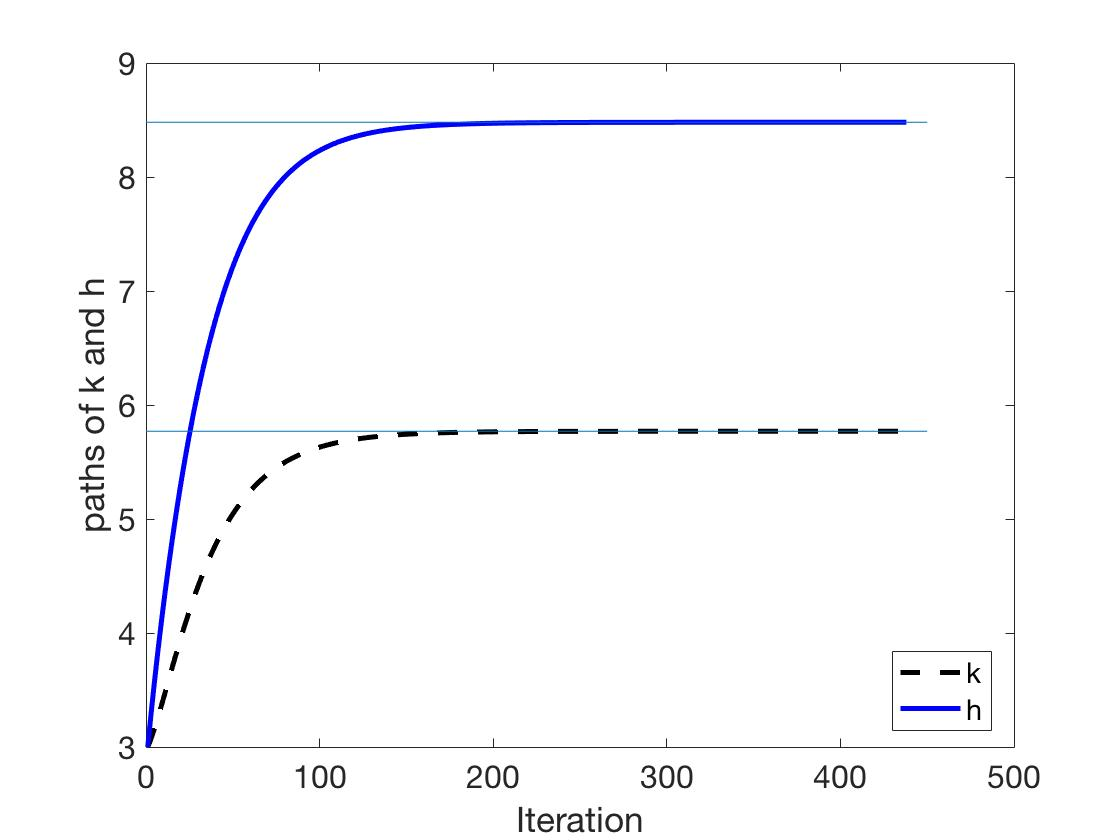
\includegraphics[width=\textwidth,height=\textheight,keepaspectratio, center]{Q2Sub6.jpg} 
\caption{Paths of $k^*$ and $h^*$}
\end{figure}
\noindent Both variables converge to the solution at the same time/speed. Optimal allocation human capital exceeds the optimal level of capital in all iterations.\\ A possible interpretation: That the balanced growth path level of human capital is greater than the balanced growth path level of physical capital could have two (simultaneous) reasons:
\begin{enumerate}
\item Human capital has a greater marginal product compared to physical capital
\item Human capital has a lower depreciation rate than physical capital
\end{enumerate}
The reasoning behind this it that if an additional unit of human capital yields more than an additional unit of physical capital, and lasts longer than it as well, and investment in human capital is preferred over an investment in physical capital. This goes on this way until a point is reached, where an investment in human capital has the same marginal-product-to-depreciation-rate as physical capital. The investment in the two goods will increase such that their levels always give the same marginal-product-to-depreciation-rate (which implies a constant ratio of human to physical capital (which can be seen in the graph as well)) until the entire income is spent. At this point, the balanced growth path level is reached.
%Since the balanced growth path level of human capital is greater, a not-so-large share of human capital depreciates per period. Thus, a not-so-large saving is needed in order to keep human capital per efficiency unit of labor constant.
\end{document}